\chapter{Effects of Patient-Specific Variability in Inconsistent End-Expiratory Diaphragm Position On the Quantification of Left Ventricular Cardiac Strains}

\section{Background}
	Cardiac strains describe the deformation of myocardial tissue during contraction and relaxation. Measures of cardiac strains have been shown to be superior predictors of outcomes, such as mortality, compared to traditional measures of cardiac function or traditional clinical risk factors alone \cite{Stanton2009}. Imaging can non-invasively assess cardiac strains using echocardiographic techniques such as speckle tracking \cite{Amundsen2006} and cardiovascular magnetic resonance (MR) techniques such as myocardial feature tracking \cite{Hor2010}, myocardial tissue tagging \cite{Axel1989,Zerhouni1988}, phase velocity mapping \cite{Pelc1994}, strain encoding \cite{Osman2001}, and displacement encoding with stimulated echoes (DENSE) \cite{Aletras1999b,Aletras1999c}.

	Peak strains vary longitudinally throughout the left ventricle \cite{Kuijer2002,Moore2000,Young1994a,Feng2009,NasiraeiMoghaddam2010,Donekal2013a,Suever2017}. For example, previous studies have shown that left ventricular radial, circumferential, and longitudinal strains vary between the base and apex by up to 14\%, 5\%, and 5\% (absolute), respectively \cite{Kuijer2002,Moore2000,Young1994a,Feng2009,NasiraeiMoghaddam2010,Donekal2013a,Suever2017}. Cardiac MR images are often acquired during end-expiratory breath-holds to minimize respiratory motion artifacts. However, it is often difficult to achieve consistency in end-expiratory diaphragm position between successive breath holds, and variations of 4 to 13 mm are normal \cite{Liu1993,Wang1995a,Taylor1997a,Holland1998c,Fischer2006a}. Inconsistent end-expiratory positions will impact the position of the heart with respect to the imaging plane (Figure~\ref{fig:diaphragmTranslation}). For example, previous studies have reported short-axis and long-axis through-plane displacements of up to 14 mm due to displacement of diaphragm position between breath-holds \cite{Slomka2007,Swingen2003}, and other studies have reported that the superior/inferior position of the heart can displace 55-92\% of the displacement of the diaphragm position \cite{Wang1995b,McLeish2002}. Because peak strains vary throughout the left ventricle, we hypothesize that translation of the heart with respect to the imaging plane to result in differences and variability in measured strains.

	To our knowledge, no study has evaluated the sensitivity of cardiac strains to natural end-expiratory position variability. This is an important knowledge gap, especially since the use of cardiac strains is increasing dramatically both in research and clinical practice. The purpose of this study was to determine if normal inconsistency in end-expiratory position significantly affects the quantification of cardiac strains and therefore results in higher variability in measured cardiac strains compared to strains measured at a consistent end-expiratory position.
	
	\begin{figure} 
		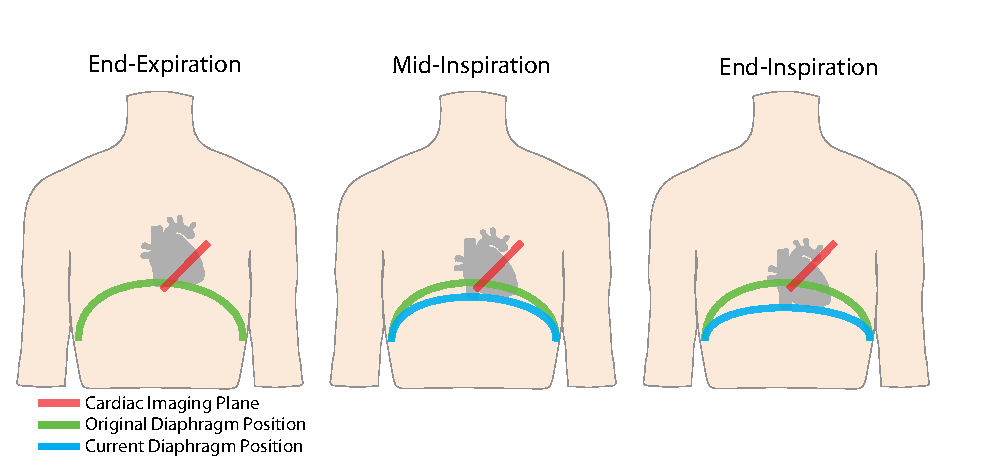
\includegraphics{figures/strainpaper/Fig1-range_of_diaphragm_position_breathing}
		\caption[During respiration, diaphragm motion causes the heart to translate a significant distance while the imaging plane remains fixed]{\textbf{During respiration, diaphragm motion causes the heart to translate a significant distance while the imaging plane remains fixed.}}
		\label{fig:diaphragmTranslation}
	\end{figure}

\section{Methods}

\subsection{Subjects}
	The study protocol was approved by the local Institutional Review Board. Ten healthy volunteers with no known cardiovascular disease or chronic illnesses and 7 patients with a history of heart disease (known diagnosis of heart failure, cardiomyopathy, or myocardial infarction) provided written informed consent. Image acquisitions were performed on a 3T Siemens Tim Trio (Siemens Healthcare, Erlangen, Germany) scanner with a 6-element chest coil and a 24-element spine coil.

\subsection{Quantification of Inconsistent End-Expiratory Positions}
	To determine the inconsistency in end-expiratory positions for each subject, a respiratory navigator sequence measured the diaphragm position (Figure~\ref{fig:navGatingExplanationCartoon}) during 10 consecutive breath-holds. During each breath-hold, the diaphragm position was imaged three times per second over a period of 10 seconds for 30 total measurements. No cardiac image data were collected during these acquisitions. The mode of the 30 diaphragm positions defined the measured end-expiratory position of that breath-hold. The patient-specific minimum, middle, and maximum end-expiratory positions were defined from the series of 10 breath-holds (Figure~\ref{fig:translatedAccWindowBlue}).
	
	\begin{figure} 
		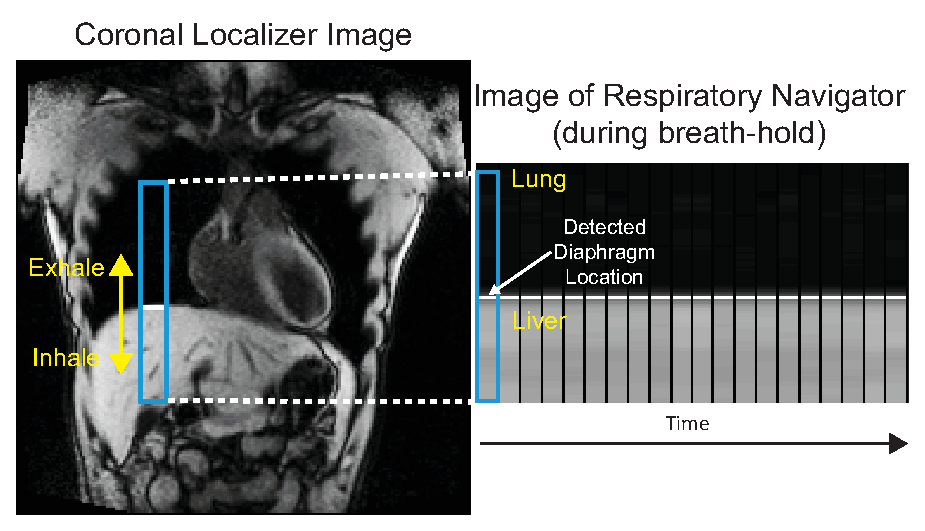
\includegraphics{figures/strainpaper/Fig2-navigator_gating_explanation_NoAccWin}
		\caption[Respiratory navigator gating]{\textbf{Respiratory navigator gating.} (Left) The diaphragm position was measured at the high-contrast interface between the lung (dark) and the liver (bright). (Right) Image of a measured diaphragm position over time during a breath-hold.}
		\label{fig:navGatingExplanationCartoon}
	\end{figure}
	
	\begin{figure} 
		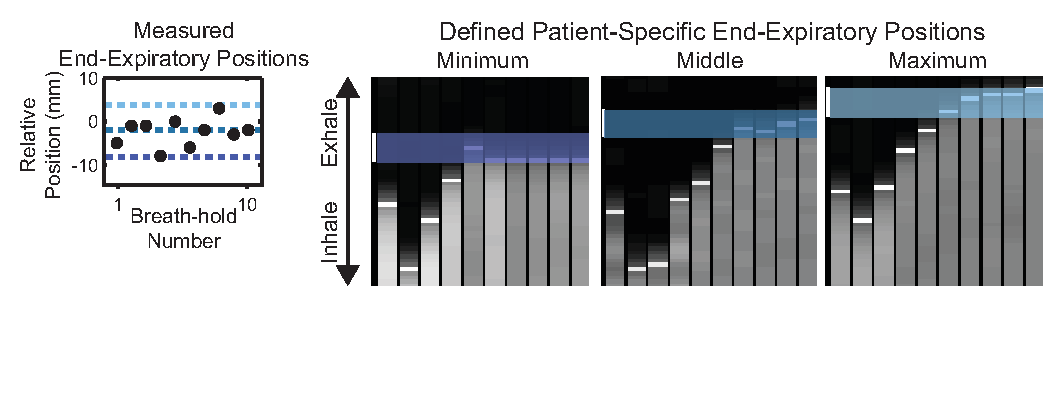
\includegraphics{figures/strainpaper/Fig3-definedTranslatedAccWindow}
		\caption[A respiratory navigator was used to measure end-expiratory positions to define the patient-specific minimum, middle, and maximum end-expiratory positions]{\textbf{A respiratory navigator was used to measure end-expiratory positions to define the patient-specific minimum, middle, and maximum end-expiratory positions.} The minimum position was defined as being closer to the end-inspiratory position while the maximum position was defined as being closer to the end-expiratory position.}
		\label{fig:translatedAccWindowBlue}
	\end{figure}
	
\subsection{DENSE Acquisition}
	For each subject, navigator-gated 2D spiral cine DENSE in 2-chamber and 4-chamber long-axis and basal, mid-ventricular, and apical short-axis orientations of the left ventricle were acquired four times. Specifically, all image orientations were acquired with the navigator acceptance window prescribed at the patient-specific maximum and minimum end-expiratory positions, and twice in the middle position to quantify variability in strain independent of end-expiratory position variability (Figure~\ref{fig:translatedAccWindowBlue}). A navigator feedback system, which used an angled mirror and projector screen placed at the back of the scanner bore, was used to facilitate quicker acquisitions by enabling subjects to view the navigator acceptance window position in real-time during image acquisition \cite{Hamlet2016a}. For each end-expiratory position, all image orientations were acquired within a single navigator-gated scan.
	
	Prospective ECG gating was used during DENSE acquisitions. The number of cardiac phases ranged from 31 to 49 and varied based on subject heart rate. Additional DENSE imaging parameters included: spiral interleaves = 6, FOV~=~ 360x360 mm$^2$, pixel spacing = 2.8x2.8 mm$^2$, slice thickness = 8 mm, TE = 1.1 ms, TR = 17 ms, variable flip angle = 20$^{\circ}$, displacement encoding = 0.06 cyc/mm \cite{Wehner2015a}, through-plane dephasing = 0.08 cyc/mm \cite{Zhong2006a}, CSPAMM echo suppression \cite{Kim2004}, and view sharing. A dual-navigator strategy was used, requiring the diaphragm to be within the navigator acceptance window ($\pm$3 mm) both before and after the data acquisition during each R-R interval \cite{Hamlet2016}.
	
\subsection{DENSE Post-Processing}
	DENSE image data were analyzed using the open-source software, \textit{DENSEanalysis} \cite{Gilliam2016a}. For each image orientation, the left ventricular myocardium was manually delineated using epicardial and endocardial contours and an end-diastolic and end-systolic cardiac phase \cite{Suever2014}. Post-processing and segmentation were performed as described by Suever et al. \cite{Suever2014}. Seed points indicating unwrapped phase data were manually selected, and a path-following algorithm was used to unwrap the displacement-encoded phase data. The resulting displacement trajectories were further processed by applying spatial smoothing and temporal fitting as previously described \cite{Spottiswoode2007}.
	
	Two-dimensional Lagrangian strains were computed from the smoothed trajectories over the entire cardiac cycle. Radial and circumferential strains were computed from the short-axis images and longitudinal strain was computed from the long-axis images. Global peak strains were calculated by averaging the mean strain curves of all the myocardial segments and identifying the peak of the global mean curve. Regional peak strains were computed by averaging the strain curves from all the myocardial segments for a given region and identifying the peak of the regional curve. Segmental peak strains were computed by identifying the peak of the strain curve for each myocardial segment. For peak longitudinal strain computation, pixels within 10\% of left ventricular longitudinal length from the most basal and apical regions were excluded because of the increased noise which is typically observed in the strain curves in those regions. Peak strain was defined as positive for thickening (radial) and negative for shortening (circumferential and longitudinal).
	
\subsection{Statistics}
	Statistical analyses were performed using R version 3.2.2 (R Foundation for Statistical Computing, Vienna, Austria). All continuous variables were expressed as mean $\pm$ standard deviation or range. Cardiac strains were tested for normality using a Shapiro-Wilk test.
	
	To quantify mean differences in cardiac strains due to inconsistent end-expiratory positions (minimum, middle, and maximum positions), cardiac strains were compared between the patient-specific acceptance window positions using a two-way analysis of variance (ANOVA) with repeated measures with group (healthy vs patient) and acceptance window position as the independent factors. A Scheirer-Ray-Hare test was used for data determined to be non-normally distributed \cite{Dytham2011}. Using the results of the two-way ANOVA or Scheirer-Ray-Hare test, the interaction between group and acceptance window position on cardiac strains was determined. If there was no interaction between group and acceptance window position, the groups were combined and mean differences due to inconsistent end-expiratory positions were quantified by comparing cardiac strains between acceptance window positions using a one-way ANOVA with repeated measures with acceptance window position as the independent factor. A Friedman test was used for data determined to be non-normally distributed \cite{Dytham2011}.
	
	To quantify variability due to inconsistent end-expiratory positions, the standard deviations of strains were compared between the inconsistent positions (maximum, middle, and minimum) and consistent positions (two acquisitions at the middle position) using a Student’s t-test. For all statistical tests, significance was defined as p $<$ 0.05. Bland-Altman analysis \cite{Bland1986} was used to assess the reproducibility of each measurement using inter-test 95\% limits of agreement defined using the two measurements from the middle position. Inconsistency in end-expiratory position across ten separate breath-holds for each subject was reported using both ranges and standard deviations from the ten breath-holds, and these values were compared between patients and healthy controls.
	
	Power analyses were performed to quantify the ability of this study to detect meaningful differences in strain between the different end-expiratory positions. Because repeated-measures ANOVAs were used to detect differences, and because equations for power are not readily available for repeated-measures ANOVA, simulations were performed to estimate power. Specifically, for each strain, 10,000 iterations were performed. For each iteration, strain values for the minimum end-expiratory position were randomly drawn from a normal distribution using the mean and standard deviation across the subjects measured in this study.  The number of strain values drawn corresponded with the number of subjects (healthy and patients combined). For a given difference to detect, $\delta$, values at the two other end-expiratory positions were calculated by adding $\delta/2$ and $\delta$ to the values at the minimum position. Measurement variability was then added to those two end-expiratory positions by drawing random values from a normal distribution with zero mean and a standard deviation equal to the measured average standard deviation of the differences between any two positions. In this manner, each iteration simulated a mean difference of $\delta$ between the minimum and maximum breath-hold positions and included typical inter-test measurement variability. The percentage of iterations for which a repeated-measures ANOVA yielded a significant result (p $<$  0.05) was the estimate of power. The 95\% confidence interval of that estimate was calculated from the normal approximation to the binomial distribution with N = 10,000. The values of $\delta$ that yielded at least 80\% power were reported separately for global and regional strains.

\section{Results}
	Ten healthy volunteers (Age: 22 $\pm$ 6 years, 60\% female) along with 7 patient volunteers (Age: 57 $\pm$ 8 years, 43\% female) were recruited. One healthy subject was excluded due to movement during imaging, so data from the remaining 9 healthy subjects are reported. Data from the basal and apical DENSE images of these subjects were previously used to assess the variability of left ventricular torsion \cite{Hamlet2017}.
	
\subsection{Inconsistent End-Expiratory Positions}
	As previously reported \cite{Hamlet2017}, the average range of end-expiratory positions were not significantly different (p~=~0.94) between the healthy (10.1 $\pm$ 4.8~mm) and patient (10.3 $\pm$ 4.2~mm) groups (total range of 4-–19~mm). Since range is sensitive to outliers, the standard deviation of end-expiratory position was also compared between groups, and similarly there were no significant differences (3.1 $\pm$ 1.3~mm vs 3.4 $\pm$ 1.7~mm, p~=~0.70) \cite{Hamlet2017}.
	
\subsection{Differences and Variability in Peak Strains}
	There was no interaction between group (healthy vs patient) and navigator acceptance window position for peak strains (Table~\ref{table:strainDifferencesPosition}), thus the remaining analyses were performed with all subjects combined. Neither global, regional, nor segmental peak strains were significantly different as a function of acceptance window position (Table~\ref{table:strainDifferencesPosition}, Tables~\ref{table:SegmentalEccStrainDiff}, and ~\ref{table:SegmentalErrStrainDiff}). Moreover, the differences in mean strain between any two acceptance window positions were each smaller than their corresponding inter-test 95\% limits of agreement (Table~\ref{table:strainDifferencesPosition}). For example, mean global circumferential strain across acceptance window positions ranged from -16\% to -17\%; the difference was 1\%, which is smaller than the corresponding inter-test 95\% limits of agreement of $\pm$1.7\% (Table~\ref{table:strainDifferencesPosition}). Finally, the standard deviations in peak strains were not significantly different between inconsistent (minimum, middle, and maximum) and consistent (repeated measurements at middle position) acceptance window positions for all subjects combined (Table~\ref{table:strainInconsVsCons}). With at least 80\% power, this study had the ability to detect strain differences of 4.7\%, 1.0\%, and 1.7\% (absolute) between end-expiratory positions for global radial, circumferential, and longitudinal strain, respectively (Table~\ref{table:strainDifferencesPower}). Additionally, this study had at least 80\% power to detect differences of 8.9\%, 2.2\% and 2.6\% for regional radial, circumferential, and longitudinal strain, respectively (Table~\ref{table:strainDifferencesPower}).
	
	%Table 2.1
	\begin{table}
		\centering
		\caption[Global and regional peak strains (mean ± standard deviation) from the three acceptance window positions (minimum, middle, and maximum) for all subjects combined]{\textbf{Global and regional peak strains (mean ± standard deviation) from the three acceptance window positions (minimum, middle, and maximum) for all subjects combined.}}
		\label{table:strainDifferencesPosition}
		\begin{tabular}{c c c c c c c}
			% Table Head
			\toprule
			\multirow{2}{*}{\textbf{Measurement}} & \multicolumn{3}{c}{\textbf{Acceptance Window Position}} & \multirow{2}{*}{\textbf{p-value$\dagger$}} & \multirow{2}{*}{\textbf{95\% LoA}}    & \multirow{2}{*}{\textbf{p-value$\ddagger$}} \\ 
			                                      & \textbf{Minimum} & \textbf{Middle} & \textbf{Maximum} & & &    \\
			\midrule
			% Table Body
			% Radial Strain
			\multicolumn{1}{l}{Radial Strain (\%)} & & & & & &       								              \\
			\multicolumn{1}{r}{Global}  	  & 29 $\pm$ 12 & 29 $\pm$ 12 & 30 $\pm$ 13 & 0.95 & $\pm$7.9  & 0.99 \\
			\multicolumn{1}{r}{Base}  		  & 37 $\pm$ 15 & 35 $\pm$ 14 & 37 $\pm$ 14 & 0.95 & $\pm$13.1 & 0.89 \\
			\multicolumn{1}{r}{Mid-Ventricle} & 28 $\pm$ 11 & 29 $\pm$ 14 & 28 $\pm$ 13 & 0.77 & $\pm$10.4 & 0.51 \\
			\multicolumn{1}{r}{Apex}  		  & 26 $\pm$ 12 & 27 $\pm$ 10 & 29 $\pm$ 16 & 0.78 & $\pm$15.8 & 0.79 \\
			% Circumferential Strain
			\multicolumn{1}{l}{Circum. Strain (\%)} & & & & & &								                      \\
			\multicolumn{1}{r}{Global}  	  & -16 $\pm$ 4 & -17 $\pm$ 4 & -17 $\pm$ 5 & 0.57 & $\pm$1.7  & 0.65 \\
			\multicolumn{1}{r}{Base}  		  & -15 $\pm$ 4	& -15 $\pm$ 4 & -15 $\pm$ 4 & 0.83 & $\pm$3.6  & 0.71 \\
			\multicolumn{1}{r}{Mid-Ventricle} & -16 $\pm$ 4 & -17 $\pm$ 4 & -17 $\pm$ 4 & 0.17 & $\pm$2.1  & 0.78 \\	   			\multicolumn{1}{r}{Apex}          & -19 $\pm$ 5 & -19 $\pm$ 5 & -19 $\pm$ 5 & 0.98 & $\pm$4.6  & 0.93 \\
			% Longitudinal Strain
			\multicolumn{1}{l}{Long. Strain (\%)} & & & & & &								    				  \\
			\multicolumn{1}{r}{Global}        & -12 $\pm$ 4 & -12 $\pm$ 3 & -13 $\pm$ 4 & 0.44 & $\pm$3.2 & 0.48  \\
			\multicolumn{1}{r}{2ch}  		  & -13 $\pm$ 3 & -12 $\pm$ 3 & -13 $\pm$ 4 & 0.94 & $\pm$6.2 & 0.75  \\
			\multicolumn{1}{r}{4ch}  		  & -12 $\pm$ 4 & -13 $\pm$ 4 & -13 $\pm$ 4 & 0.84 & $\pm$4.1 & 0.38  \\ 
			\bottomrule
			\multicolumn{7}{l}{$\dagger$Results from test comparing acceptance window positions} \\
			\multicolumn{7}{l}{$\ddagger$Results from test comparing interaction between group (healthy vs patient) and acceptance} \\
			\multicolumn{7}{l}{window position}
		\end{tabular}
	\end{table}

	%Table 2.2
	\begin{sidewaystable}
		\centering
		\caption[Segmental circumferential strain (\%, mean $\pm$ standard deviation) from the three acceptance window positions (minimum, middle, and maximum) for all subjects combined]{\textbf{Segmental circumferential strain (\%, mean $\pm$ standard deviation) from the three acceptance window positions (minimum, middle, and maximum) for all subjects combined.}}
		\label{table:SegmentalEccStrainDiff}
		\begin{tabular}{ccccccccccccc}
			\toprule
			% Top Headings
			\multirow{2}{*}{} & \multicolumn{2}{c}{Anterior} & \multicolumn{2}{c}{Anteroseptal} & \multicolumn{2}{c}{Inferoseptal} &
			\multicolumn{2}{c}{Inferior} & \multicolumn{2}{c}{Inferolateral} & \multicolumn{2}{c}{Anterolateral}\\
			% Second from top headings
			& \textbf{Strain} & \textbf{P} & \textbf{Strain} & \textbf{P} & \textbf{Strain} & \textbf{P} &
			\textbf{Strain} & \textbf{P} & \textbf{Strain} & \textbf{P} & \textbf{Strain} & \textbf{P} \\
			\midrule
			
			% Basal Data
			\multicolumn{13}{c}{\textbf{Basal}} \\
			\midrule
			\textbf{Max} & -16$\pm$5 & \multirow{3}{*}{0.99} & -14$\pm$5 & \multirow{3}{*}{1.0} & -14$\pm$5 & \multirow{3}{*}{0.95}
			& -15$\pm$5 & \multirow{3}{*}{0.91} & -19$\pm$6 & \multirow{3}{*}{0.88} & -19$\pm$5 & \multirow{3}{*}{0.76} \\
			\textbf{Mid} & -16$\pm$3 &                       & -13$\pm$5 &                       & -15$\pm$5 & 
			& -15$\pm$5 &                       & -18$\pm$5 &                       & -19$\pm$5 &                       \\
			\textbf{Min} & -15$\pm$4 &                       & -13$\pm$5 &                       & -15$\pm$4 & 
			& -15$\pm$5 &                       & -19$\pm$6 &                       & -18$\pm$4 &  \\ 
			\midrule
			
			% Mid-Ventricular Data
			\multicolumn{13}{c}{\textbf{Mid-Ventricular}} \\
			\midrule
			\textbf{Max} & -17$\pm$5 & \multirow{3}{*}{0.93} & -14$\pm$5 & \multirow{3}{*}{0.83} & -13$\pm$5 & \multirow{3}{*}{0.87}
			& -17$\pm$5 & \multirow{3}{*}{0.93} & -22$\pm$6 & \multirow{3}{*}{1.0}  & -20$\pm$6 & \multirow{3}{*}{0.81} \\
			\textbf{Mid} & -17$\pm$5 &                       & -14$\pm$4 &                       & -14$\pm$4 & 
			& -18$\pm$5 &                       & -21$\pm$4 &                       & -21$\pm$6 &                       \\
			\textbf{Min} & -17$\pm$6 &                       & -14$\pm$4 &                       & -13$\pm$4 & 
			& -17$\pm$3 &                       & -20$\pm$5 &                       & -21$\pm$6 & \\ 
			\midrule
			
			% Apical Data
			\multicolumn{13}{c}{\textbf{Apical}} \\
			\midrule
			\textbf{Max} & -18$\pm$5 & \multirow{3}{*}{0.66} & -15$\pm$6 & \multirow{3}{*}{0.99} & -17$\pm$6 & \multirow{3}{*}{0.79}
			& -20$\pm$6 & \multirow{3}{*}{0.98} & -23$\pm$7 & \multirow{3}{*}{0.84} & -22$\pm$6 & \multirow{3}{*}{0.99} \\
			\textbf{Mid} & -18$\pm$5 &                       & -15$\pm$5 &                       & -17$\pm$6 & 
			& -20$\pm$6 &                       & -23$\pm$6 &                       & -22$\pm$7 &                       \\
			\textbf{Min} & -18$\pm$6 &                       & -15$\pm$5 &                       & -16$\pm$6 & 
			& -21$\pm$6 &                       & -24$\pm$6 &                       & -21$\pm$7 & \\ 
			\bottomrule
			\multicolumn{13}{l}{P-values indicate results from test comparing acceptance window positions.}
		\end{tabular}
	\end{sidewaystable}
	
	%Table 2.3
	\begin{sidewaystable}
		\centering
		\caption[Segmental radial strain (\%, mean $\pm$ standard deviation) from the three acceptance window positions (minimum, middle, and maximum) for all subjects combined]{\textbf{Segmental radial strain (\%, mean $\pm$ standard deviation) from the three acceptance window positions (minimum, middle, and maximum) for all subjects combined.}}
		\label{table:SegmentalErrStrainDiff}
		\begin{tabular}{ccccccccccccc}
			\toprule
			% Top Headings
			\multirow{2}{*}{} & \multicolumn{2}{c}{Anterior} & \multicolumn{2}{c}{Anteroseptal} & \multicolumn{2}{c}{Inferoseptal} &
			\multicolumn{2}{c}{Inferior} & \multicolumn{2}{c}{Inferolateral} & \multicolumn{2}{c}{Anterolateral}\\
			% Second from top headings
			& \textbf{Strain} & \textbf{P} & \textbf{Strain} & \textbf{P} & \textbf{Strain} & \textbf{P} &
			\textbf{Strain} & \textbf{P} & \textbf{Strain} & \textbf{P} & \textbf{Strain} & \textbf{P} \\
			\midrule
			
			% Basal Data
			\multicolumn{13}{c}{\textbf{Basal}} \\
			\midrule
			\textbf{Max} & 37$\pm$20 & \multirow{3}{*}{0.78} & 36$\pm$16 & \multirow{3}{*}{0.61} & 40$\pm$20 & \multirow{3}{*}{0.53}
			& 43$\pm$23 & \multirow{3}{*}{0.77} & 47$\pm$29 & \multirow{3}{*}{0.94} & 41$\pm$21 & \multirow{3}{*}{0.64} \\
			\textbf{Mid} & 40$\pm$21 &                       & 41$\pm$18 &                       & 37$\pm$14 & 
			& 36$\pm$21 &                       & 47$\pm$31 &                       & 44$\pm$24 &                       \\
			\textbf{Min} & 38$\pm$18 &                       & 38$\pm$17 &                       & 37$\pm$18 & 
			& 40$\pm$22 &                       & 51$\pm$29 &                       & 46$\pm$28 &  \\ 
			\midrule
			
			% Mid-Ventricular Data
			\multicolumn{13}{c}{\textbf{Mid-Ventricular}} \\
			\midrule
			\textbf{Max} & 28$\pm$17 & \multirow{3}{*}{0.94} & 33$\pm$24 & \multirow{3}{*}{0.44} & 34$\pm$15 & \multirow{3}{*}{0.88}
			& 32$\pm$15 & \multirow{3}{*}{0.96} & 36$\pm$32 & \multirow{3}{*}{0.83} & 32$\pm$17 & \multirow{3}{*}{0.49} \\
			\textbf{Mid} & 31$\pm$19 &                       & 35$\pm$19 &                       & 31$\pm$13 & 
			& 33$\pm$24 &                       & 38$\pm$29 &                       & 33$\pm$18 &                       \\
			\textbf{Min} & 30$\pm$19 &                       & 36$\pm$14 &                       & 36$\pm$16 & 
			& 31$\pm$21 &                       & 35$\pm$24 &                       & 28$\pm$17 &  \\ 
			\midrule
			
			% Apical Data
			\multicolumn{13}{c}{\textbf{Apical}} \\
			\midrule
			\textbf{Max} & 28$\pm$24 & \multirow{3}{*}{0.72} & 36$\pm$37 & \multirow{3}{*}{0.87} & 41$\pm$21 & \multirow{3}{*}{0.83}
			& 41$\pm$37 & \multirow{3}{*}{0.20} & 31$\pm$23 & \multirow{3}{*}{0.84} & 27$\pm$16 & \multirow{3}{*}{0.69} \\
			\textbf{Mid} & 23$\pm$12 &                       & 31$\pm$13 &                       & 39$\pm$20 & 
			& 40$\pm$20 &                       & 27$\pm$17 &                       & 26$\pm$15 &                       \\
			\textbf{Min} & 25$\pm$15 &                       & 35$\pm$24 &                       & 40$\pm$27 & 
			& 34$\pm$24 &                       & 29$\pm$20 &                       & 33$\pm$16 &  \\ 
			\bottomrule
			\multicolumn{13}{l}{P-values indicate results from test comparing acceptance window positions.}
		\end{tabular}
	\end{sidewaystable}

    %Table 2.4
	\begin{table}
		\centering
		\caption[Standard deviation of global and regional peak strains across inconsistent (maximum, middle, minimum) and consistent (middle and repeated middle) acceptance window positions]{\textbf{Standard deviation of global and regional peak strains across inconsistent (maximum, middle, minimum) and consistent (middle and repeated middle) acceptance window positions.} Values reported as mean ± standard deviation.}
		\label{table:strainInconsVsCons}
		\begin{tabular}{c c c c}
			% Table Head
			\toprule
			\multirow{2}{*}{\textbf{Measurement}} & \multicolumn{2}{c}{\textbf{Acceptance Window Positioning}} & \multirow{2}{*}{\textbf{p-value}}  \\ 
			& \textbf{Inconsistent} & \textbf{Consistent} & \\
			\midrule
			% Table Body
			% Radial Strain
			\multicolumn{1}{l}{Radial Strain (\%)} & & &   \\
			\multicolumn{1}{r}{Global}  	  & 3.2 $\pm$ 1.7 &	2.3 $\pm$ 1.8 &	0.17 \\
			\multicolumn{1}{r}{Base}  		  & 4.9 $\pm$ 2.5 & 3.5 $\pm$ 3.3 & 0.18 \\
			\multicolumn{1}{r}{Mid-Ventricle} & 4.3 $\pm$ 2.5 & 2.5 $\pm$ 2.8 & 0.10 \\
			\multicolumn{1}{r}{Apex}  		  & 5.7 $\pm$ 4.1 & 4.3 $\pm$ 3.9 & 0.16 \\
			% Circumferential Strain
			\multicolumn{1}{l}{Circumferential Strain (\%)} & & &	\\
			\multicolumn{1}{r}{Global}  	  & 0.7 $\pm$ 0.4 & 0.5 $\pm$ 0.3 & 0.10 \\
			\multicolumn{1}{r}{Base}  		  & 1.0 $\pm$ 0.5 & 1.1 $\pm$ 0.7 & 0.41 \\
			\multicolumn{1}{r}{Mid-Ventricle} & 0.7 $\pm$ 0.3 & 0.6 $\pm$ 0.5 & 0.55 \\	   			
			\multicolumn{1}{r}{Apex}          & 1.4 $\pm$ 0.9 & 1.4 $\pm$ 0.9 & 0.95 \\
			% Longitudinal Strain
			\multicolumn{1}{l}{Longitudinal Strain (\%)} & & &								    				  \\
			\multicolumn{1}{r}{Global}        & 1.1 $\pm$ 0.7 & 0.8 $\pm$ 0.9 & 0.27  \\
			\multicolumn{1}{r}{2ch}  		  & 1.4 $\pm$ 1.1 & 1.5 $\pm$ 1.6  & 0.89  \\
			\multicolumn{1}{r}{4ch}  		  & 1.4 $\pm$ 1.6 & 1.2 $\pm$ 0.9  & 0.72  \\ 
			\bottomrule
		\end{tabular}
	\end{table}

	%Table 2.5
	\begin{table}
		\centering
		\caption[Power analyses for study's ability to detect a difference in global and regional strain between different end-expiratory positions]{\textbf{Power analyses for study's ability to detect a difference in global and regional strain between different end-expiratory positions.}}
		\label{table:strainDifferencesPower}
		\begin{tabular}{c c c}
			% Table Head
			\toprule
			\multirow{2}{*}{\textbf{Measurement}} & \multirow{2}{*}{\textbf{Power (\%)}} & \textbf{Difference To Detect}  \\
			 & & \textbf{(absolute, \%)}\\
			\midrule
			% Table Body
			% Radial Strain
			\multicolumn{1}{l}{Radial Strain (\%)} & &                                 \\
			\multicolumn{1}{r}{Global}  	  & 80.9 $\pm$ 0.8 & 4.7                   \\
			\multicolumn{1}{r}{Base}  		  & 96.1 $\pm$ 0.4 & \multirow{3}{*}{8.9}  \\
			\multicolumn{1}{r}{Mid-Ventricle} & 98.4 $\pm$ 0.2 &                       \\
			\multicolumn{1}{r}{Apex}  		  & 80.2 $\pm$ 0.8 &                       \\
			% Circumferential Strain
			\multicolumn{1}{l}{Circumferential Strain (\%)} & &                        \\
			\multicolumn{1}{r}{Global}  	  & 80.5 $\pm$ 0.8 & 1.0                   \\
			\multicolumn{1}{r}{Base}  		  & 99.6 $\pm$ 0.1 & \multirow{3}{*}{2.2}  \\
			\multicolumn{1}{r}{Mid-Ventricle} & 100 $\pm$ 0.0  &                       \\
			\multicolumn{1}{r}{Apex}  		  & 80.6 $\pm$ 0.8 &                       \\
			% Longitudinal Strain
			\multicolumn{1}{l}{Longitudinal Strain (\%)} & & 	    				   \\
			\multicolumn{1}{r}{Global}        & 80.0 $\pm$ 0.8 &  1.7                  \\
			\multicolumn{1}{r}{2ch}  		  & 95.0 $\pm$ 0.4 &  \multirow{2}{*}{2.6} \\
			\multicolumn{1}{r}{4ch}  		  & 80.5 $\pm$ 0.8 &     				   \\ 
			\bottomrule
		\end{tabular}
	\end{table}

\section{Discussion}
	Quantification of cardiac strains typically requires a series of image acquisitions performed during end-expiratory breath-holds. This study explored the effects of inconsistent end-expiratory positions on the quantification of left ventricular cardiac strains. The results of the study showed that 1) inconsistent end-expiratory positions had minimal effect on the quantification of global and regional peak strains compared to inter-test variability for a given imaging location; and 2) the variability of global and regional peak strains was similar between inconsistent and consistent end-expiratory positions. Importantly, these findings provide assurance that the measurement of cardiac strains is relatively robust with respect to inconsistent end-expiratory positions.
	
	Peak strains vary throughout the left ventricle. For example, we found that the magnitude of circumferential strain was 2\% (absolute) higher in the apical region than the base--in agreement with previous studies \cite{Kuijer2002,Moore2000,Young1994a,Feng2009,NasiraeiMoghaddam2010,Donekal2013a}--and radial strain was 9\% (absolute) higher in the basal region than the apex. Due to these strain gradients, we hypothesized that the displacement of the heart due to motion of the diaphragm with respect to the imaging plane would create differences in measured strains. For example, we might expect that radial strains for the maximum end-expiratory position (i.e., maximal exhalation) would be lower in magnitude compared to the minimum end-expiratory position due to the heart being imaged more apically. We also might expect this to manifest as higher variability in strains across different end-expiratory positions compared to consistent end-expiratory positions. The likely explanation for finding that there is no difference in strains between end-expiratory positions is that, because the longitudinal axis of the heart (base to apex) is not necessarily perpendicular to the diaphragm plane, a 10 mm translation in the diaphragm position does not directly correspond with a 10 mm translation of the heart through the imaging plane.
	
	Previous studies suggest that regions of the heart could displace at least 3 and possibly up to 14 mm through the fixed imaging plane between breath-holds \cite{Slomka2007,Swingen2003,Wang1995b,McLeish2002}. Our study had an average range of end-expiratory diaphragm position between breath-holds of approximately 10 mm, which is consistent with previous studies. Since the imaging slice thickness is 8 mm, even with a 14 mm through-plane displacement, there is likely not much difference in the acquired data from the imaged heart locations compared to the imaging plane location. Overall, since there were no significant differences in peak global, regional, and segmental strains between end-expiratory positions, patient end-expiratory diaphragm position does not have to be monitored when performing breath-hold DENSE acquisition for single image analyses.
	
	This study’s goal was to quantify the effects of inconsistent end-expiratory positions on cardiac strains by computing the differences in strain between different end-expiratory positions. Thus, it was important for this study to detect meaningful strain differences between different patient-specific end-expiratory positions. This study had at least 80\% power to detect global strain differences of 4.7\%, 1.0\%, and 1.7\% and regional strain differences of 8.9\%, 2.2\%, and 2.6\%, between different end-expiratory positions for radial, circumferential, and longitudinal strain, respectively. Importantly, the study’s detectable difference was similar to or smaller than previously reported values of inter-test limits of agreement for circumferential strain and radial strain \cite{Wehner2015a}. Notably, in some regions, the power to detect a meaningful difference was much higher (close to 100\%) indicating that, in those regions, this study may have had the ability to detect even smaller than reported detectable differences.
	
	We used DENSE to investigate our hypothesis that a patient’s normal variability in end-expiratory position between image acquisitions significantly affects the quantification of cardiac strains. DENSE was chosen to test our hypothesis because it has been previously shown to have good reproducibility \cite{Haggerty2013}, can be acquired in high spatial resolution \cite{Aletras1999b,Aletras1999c}, and enables straightforward computation of cardiac strains. However, our findings should generalize to other image acquisitions that are used to derive measures of cardiac strains such as echocardiography, tagged MRI, etc.
	
	We used respiratory navigator gating to acquire the DENSE cardiac images, which reduces respiratory artifacts during image acquisition, so we could not measure the effect of inconsistent end-expiratory position during breath-holds on the derived strains. It would be beneficial to quantify the amount of end-expiratory position variability during breath-hold cardiac MR image acquisition and determine whether the magnitude of inconsistent end-expiratory positions correlates with changes in strain values. An example would be to explore whether inconsistent end-expiratory positions during a breath-hold DENSE scan causes blurring due to motion and results in lower strain magnitudes.
	
	This study examined the effects of inconsistent end-expiratory positions on cardiac strains in a small patient sample. It would be beneficial to investigate this effect in a larger patient sample who have heterogeneous contraction patterns, for example, due to post-myocardial infarction. These patients may have steeper gradients in strain across infarcted to non-infarcted tissue regions \cite{Pahlm2014}. Therefore, we cannot definitively say that the effects of inconsistent end-expiratory positions in that setting are similarly small and negligible. Future studies should investigate strain variability due to inconsistent end-expiratory positions in patients who have infarcted tissue in specific regions (e.g. anterior vs inferior).
	
	In conclusion, the quantification of peak left ventricular cardiac strains is relatively insensitive to normal variations in end-expiratory positions between image acquisitions. Since there were no differences in peak strain between end-expiratory positions, patient end-expiratory diaphragm position does not have to be monitored when performing breath-hold DENSE acquisition for single image analyses. These findings should generalize to other image acquisitions that are used to derive measures of cardiac strains.
	
	
	
